\documentclass{tufte-handout}

\title{A representation of the "Game of Life"}

\author[EF Academy]{Neel Ramani}

%\{28 March 2010} % without \date command, current date is supplied

%\geometry{showframe} % display margins for debugging page layout

\usepackage{graphicx} % allow embedded images
  \setkeys{Gin}{width=\linewidth,totalheight=\textheight,keepaspectratio}
  \graphicspath{{graphics/}} % set of paths to search for images
\usepackage{amsmath}  % extended mathematics
\usepackage{booktabs} % book-quality tables
\usepackage{units}    % non-stacked fractions and better unit spacing
\usepackage{multicol} % multiple column layout facilities
\usepackage{lipsum}   % filler text
\usepackage{fancyvrb} % extended verbatim environments
  \fvset{fontsize=\normalsize}% default font size for fancy-verbatim environments
  
  
  
 
  
  \usepackage[T1]{fontenc} % Use 8-bit encoding that has 256 glyphs
\usepackage{fourier} % Use the Adobe Utopia font for the document - comment this line to return to the LaTeX default
\usepackage[english]{babel} % English language/hyphenation
\usepackage{amsmath,amsfonts,amsthm} % Math packages
\usepackage{mathtools}% http://ctan.org/pkg/mathtools
\usepackage{etoolbox}% http://ctan.org/pkg/etoolbox
\usepackage{lipsum} % Used for inserting dummy 'Lorem ipsum' text into the template
\usepackage{units}% To use \nicefrac
\usepackage{cancel}% To use \cancel
%\usepackage{physymb}%To use r
\usepackage{sectsty} % Allows customizing section commands
\usepackage[dvipsnames]{xcolor}
\usepackage{pgf,tikz}%To draw 
\usepackage{pgfplots}%To draw 
\usetikzlibrary{shapes,arrows}%To draw 
\usetikzlibrary{patterns,fadings}
 \usetikzlibrary{decorations.pathreplacing}%To draw curly braces 
 \usetikzlibrary{snakes}%To draw 
 \usetikzlibrary{spy}%To do zoom-in
 \usepackage{setspace}%Set margins and such
 %\usepackage{3dplot}%To draw in 3D
\usepackage{framed}%To get shade behind text


\definecolor{shadecolor}{rgb}{0.8,0.7,0.2}%setting shade color
\allsectionsfont{\centering \normalfont\scshape} % Make all sections centered, the default font and small caps
  
  

  
  

% Standardize command font styles and environments
\newcommand{\doccmd}[1]{\texttt{\textbackslash#1}}% command name -- adds backslash automatically
\newcommand{\docopt}[1]{\ensuremath{\langle}\textrm{\textit{#1}}\ensuremath{\rangle}}% optional command argument
\newcommand{\docarg}[1]{\textrm{\textit{#1}}}% (required) command argument
\newcommand{\docenv}[1]{\textsf{#1}}% environment name
\newcommand{\docpkg}[1]{\texttt{#1}}% package name
\newcommand{\doccls}[1]{\texttt{#1}}% document class name
\newcommand{\docclsopt}[1]{\texttt{#1}}% document class option name
\newenvironment{docspec}{\begin{quote}\noindent}{\end{quote}}% command specification environment

\begin{document}

\maketitle% this prints the handout title, author, and date
\begin{marginfigure}%
  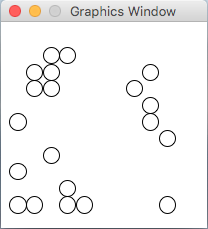
\includegraphics[width=\linewidth]{gol.png}
  \caption{This is an example of the "Conway's Game of Life".}
  \label{fig:marginfig}
\end{marginfigure}
\begin{abstract}
\noindent
\textbf{This report contains information about Conway's Game of Life.}
\end{abstract}

\normalsize
\sffamily


%this generates 1cm of vertical space
\vspace{1cm}
\section{About the Report}

This report shows:

	1){\color{red}What is} Conway's Game of Life
	
	2)What are the {\color{red}rules} of the Conway's Game of Life
	
	3){\color{red}Python Code} to create Conway's Game of Life
	
	4){\color{red}How} the code works and the {\color{red}output}




\vspace{1cm}


\large

\section{1) {\color{red}What is} Conway's Game of Life}

The {\color{blue}Game of Life}, also known simply as Life, is a cellular 
automaton devised by the British mathematician John Horton 
Conway in 1970.The "game" is a zero-player game,meaning
that its evolution is determined by its initial state, 
requiring no further input. One interacts with the Game of 
Life by creating an initial configuration and observing how 
it evolves or, for advanced players, by creating patterns 
with particular properties.


\normalsize

\section{2) What are the {\color{red}rules} of the Conway's Game of Life}

\marginnote[40pt]{\textbf{In the code shown below, the Game of Life created in Python uses the same set of rules and the grid created here depends on the input.}}


The universe of the Game of Life is an infinite two-dimensional orthogonal grid of square cells, each of which is in one of two possible states, alive or dead. Every cell interacts with its eight neighbours, which are the cells that are horizontally, vertically, or diagonally adjacent. At each step in time, the following transitions occur:

	1)Any live cell with {\color{blue}fewer than two} live neighbours dies, as if caused by under-population.
	
	2)Any live cell with {\color{blue}two or three} live neighbours lives on to the next generation.
	
	3)Any live cell with {\color{blue}more than three} live neighbours dies, as if by over-population.
	
	4)Any dead cell with {\color{blue}exactly three} live neighbours becomes a live cell, as if by reproduction.


\section{3) Python Code}

\begin{marginfigure}
  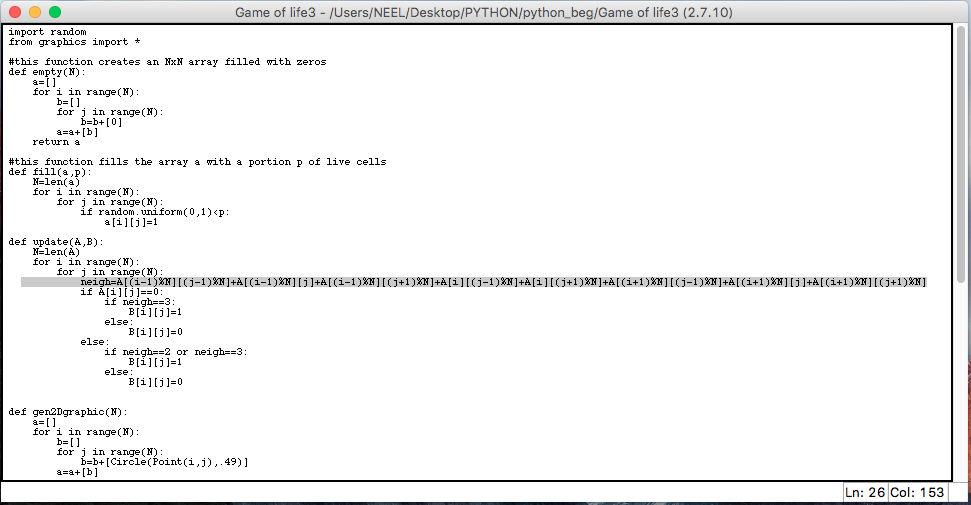
\includegraphics[width=\linewidth]{gol2.png}
  \caption{The highlighted section in the code as shown in the picture will be needed to change it in the code given below in order for it to function properly.}
  \label{fig:marginfig}
\end{marginfigure}


\marginnote[70pt]{\large{Please read the caption of the image carefully. After copying the code in Python, press enter and then you will be prompted to enter a number which will be your grid dimension.}}

\marginnote[70pt]{\large{The number you enter will be the grid size. For example, if you input the number 4, the grid created will be 4x4 size. Be sure to enter only positive integers.}}

\marginnote[70pt]{\large{The bigger the grid size is, the more computing it will take. Input of an integer \textbf{between 4 to 10} will be appropriate for a normally configured computer to show the Game of Life.}}

\begin{framed}
\begin{verbatim}

import random
from graphics import *


def empty(N):
    a=[]
    for i in range(N):
        b=[]
        for j in range(N):
            b=b+[0]
        a=a+[b]
    return a


def fill(a,p):
    N=len(a)
    for i in range(N):
        for j in range(N):
            if random.uniform(0,1)<p:
                a[i][j]=1

def update(A,B):
    N=len(A)
    for i in range(N):
        for j in range(N):
            neigh=A[(i-1)%N][(j-1)%N]+A[(i-1)%N][j]+
            		     A[(i-1)%N][(j+1)%N]+A[i][(j-1)%N]+
			                  A[i][(j+1)%N]+A[(i+1)%N][(j-1)%N]+
			                  A[(i+1)%N][j]+A[(i+1)%N][(j+1)%N]
            if A[i][j]==0:
                if neigh==3:
                    B[i][j]=1
                else:
                    B[i][j]=0
            else:
                if neigh==2 or neigh==3:
                    B[i][j]=1
                else:
                    B[i][j]=0


def gen2Dgraphic(N):
    a=[]
    for i in range(N):
        b=[]
        for j in range(N):
            b=b+[Circle(Point(i,j),.49)]
        a=a+[b]
    return a

def push(B,A):
    N=len(A)
    for i in range(N):
        for j in range(N):
            A[i][j]=B[i][j]
            
def drawArray(A,a,window):
    N=len(A)
    for i in range(N):
        for j in range(N):
            if A[i][j]==1:
                a[i][j].undraw()
                a[i][j].draw(window)
            if A[i][j]==0:
                a[i][j].undraw()

N=int(input("Enter the grid dimension  "))
win = GraphWin()
win.setCoords(-1,-1,N+1,N+1)
grid=empty(N)
grid2=empty(N)
circles=gen2Dgraphic(N)
fill(grid,0.3)

while True:
    drawArray(grid,circles,win)
    update(grid,grid2)
    push(grid2,grid)

\end{verbatim}
\end{framed}

\section{4) {\color{red}How} the code works and the {\color{red}output}}

Firstly, The code creates an array of the dimension you put in.Then, it fills the array with zero and changes random elements of the array to 1 which creates an array of 1s and 0s of a particular dimension.When this is done, the rules are applied. If there is 1 in the array, the cell is alive else the cell is dead, if the cell is alive, a circle is graphed into the window. Then it checks the neighbours and co-relates it to the rules as stated.Finally, the new array we get is graphed and then the new array is made old and the process keeps on going.

\marginnote[40pt]{This will be the first outcome when you run the code. You need to input a positive integer in order for the code to start the Game of Life with a particular grid size}

\begin{shaded}
\begin{verbatim}

>>>
Enter the grid dimension 

\end{verbatim}
\end{shaded}

After this is done, a new window will appear and the first array or the first state will be graphed and then it will {\textbf{keep updating itself}}.

\bibliography{sample-handout}
\bibliographystyle{plainnat}



\end{document}
